\documentclass[11pt,letterpaper]{article}
\PassOptionsToPackage{hyphens}{url}
\usepackage[margin=.83in,top=.8in,bottom=.8in,headheight=15pt]{geometry}
\usepackage[T1]{fontenc}
\usepackage{lmodern,amsmath,amssymb,mathtools,bm,booktabs,array,graphicx,tikz}
\usetikzlibrary{arrows.meta,positioning,calc,decorations.pathreplacing,patterns}
\definecolor{ink}{HTML}{17344D}\definecolor{accent}{HTML}{087E8B}\definecolor{pale}{HTML}{EDF5F5}\definecolor{gold}{HTML}{AD6B19}
\providecommand{\dd}{\,\mathrm{d}}\providecommand{\R}{\mathbb{R}}
\providecommand{\E}{\mathbb{E}}\providecommand{\Var}{\operatorname{Var}}
\providecommand{\Cov}{\operatorname{Cov}}\providecommand{\diag}{\operatorname{diag}}
\providecommand{\norm}[1]{\left\lVert#1\right\rVert}
\providecommand{\abs}[1]{\left|#1\right|}
\usepackage{microtype,hyperref,fancyhdr,enumitem,amsthm,sectsty,needspace}
\allsectionsfont{\raggedright}
\hypersetup{colorlinks=true,linkcolor=ink,urlcolor=accent,pdfauthor={Zan Ahmad},pdftitle={Field errors, conserved moments and correlation invariance / Lecture notes}}
\setlength{\parindent}{0pt}\setlength{\parskip}{6pt}\linespread{1.07}
\setlist{itemsep=3pt,topsep=4pt,leftmargin=*}
\emergencystretch=2em\clubpenalty=10000\widowpenalty=10000
\pagestyle{fancy}\fancyhf{}\fancyhead[L]{\small Computational Cardiology}\fancyhead[R]{\small Lecture 20}
\fancyfoot[L]{\footnotesize Zan Ahmad}\fancyfoot[R]{\footnotesize\thepage}\renewcommand{\headrulewidth}{.3pt}
\newtheorem{proposition}{Proposition}\newtheorem{theorem}{Theorem}\newtheorem{lemma}{Lemma}
\theoremstyle{definition}\newtheorem{definition}{Definition}\newtheorem{example}{Example}
\numberwithin{equation}{section}
\begin{document}
{\small\scshape Computational Cardiology\hfill Lecture 20}\par\medskip
{\raggedright\hyphenpenalty=10000\exhyphenpenalty=10000\LARGE\bfseries\color{ink} Field errors, conserved moments and correlation invariance\par}\medskip
{\small Lecture notes}\par\bigskip
A scientific result can satisfy a conserved moment or achieve perfect correlation while retaining a large field error. The final synthesis derives these counterexamples for a known heat trajectory and uses them to distinguish the mathematical statements supported by each observable.

\section{Equations and observables in a scientific argument}
\hypertarget{note-equations-and-observables-in-a-scientific-argument}{}\label{note:equations-and-observables-in-a-scientific-argument}
{\small \href{slides.html\#frame=an-observable-selects-part-of-a-solution\&step=1}{Slides for this section}}\par
A short presentation should make one question easy to assess. State the system, model, input regime and observable before showing a result. Then identify the reference and the checks that make the computation credible. Finish with the limitation that most constrains the claim and a next test that could change the conclusion. This structure helps an audience distinguish what was assumed, what was computed and what was observed independently.

The preceding models attach evidence to different mathematical objects: conservation to a balance law, valve admissibility to inequalities, wave speed to a threshold event, shape discrepancy to an alignment rule, and surrogate accuracy to an operator and input family. A presentation is precise when the claimed result names the corresponding object rather than treating every plotted agreement as the same kind of evidence.
\section{Field error and aggregate summaries}
\hypertarget{note-field-error-and-aggregate-summaries}{}\label{note:field-error-and-aggregate-summaries}
{\small \href{slides.html\#frame=two-explicit-candidate-fields-panel-1\&step=1}{Slides for this section}}\par
A field norm asks how far predicted values are from reference values across the represented domain. A mean asks about one aggregate component. Correlation asks whether centered variations align after normalization. These questions overlap only partially. A predictor can preserve a mean while losing spatial structure, or have perfect correlation while shifting every value by a substantial bias. Choosing one favorable statistic after viewing the output is not a defensible validation strategy.

The companion uses an exactly known sealed heat trajectory and constructs two explicit counterexamples. One adds 0.2 to every value. The other replaces each field with its spatial mean. These are synthetic candidate outputs, not trained-model predictions or patient data. Their simplicity makes it possible to know why a metric succeeds or fails, without invoking optimizer behavior or a hidden dataset.

At the final time, the biased candidate has absolute RMS error 0.2 and correlation essentially one. The mean-only candidate has the correct mean but loses all nonconstant structure; its field error is substantial and its correlation is undefined because its centered variance is zero. Undefined quantities are retained as missing, rather than replaced by zero or silently omitted from the discussion. A complete report explains such cases explicitly.

For vectors $p,y\in\mathbb R^N$, define $e=p-y$, mean error $\bar e=N^{-1}\sum_i e_i$ and RMS error $E=(N^{-1}\sum_i e_i^2)^{1/2}$. A relative RMS divides by $(N^{-1}\sum_i y_i^2)^{1/2}$ and is undefined when that reference norm is zero unless another convention is explicitly supplied.
\begin{center}\begin{minipage}{.98\linewidth}\centering
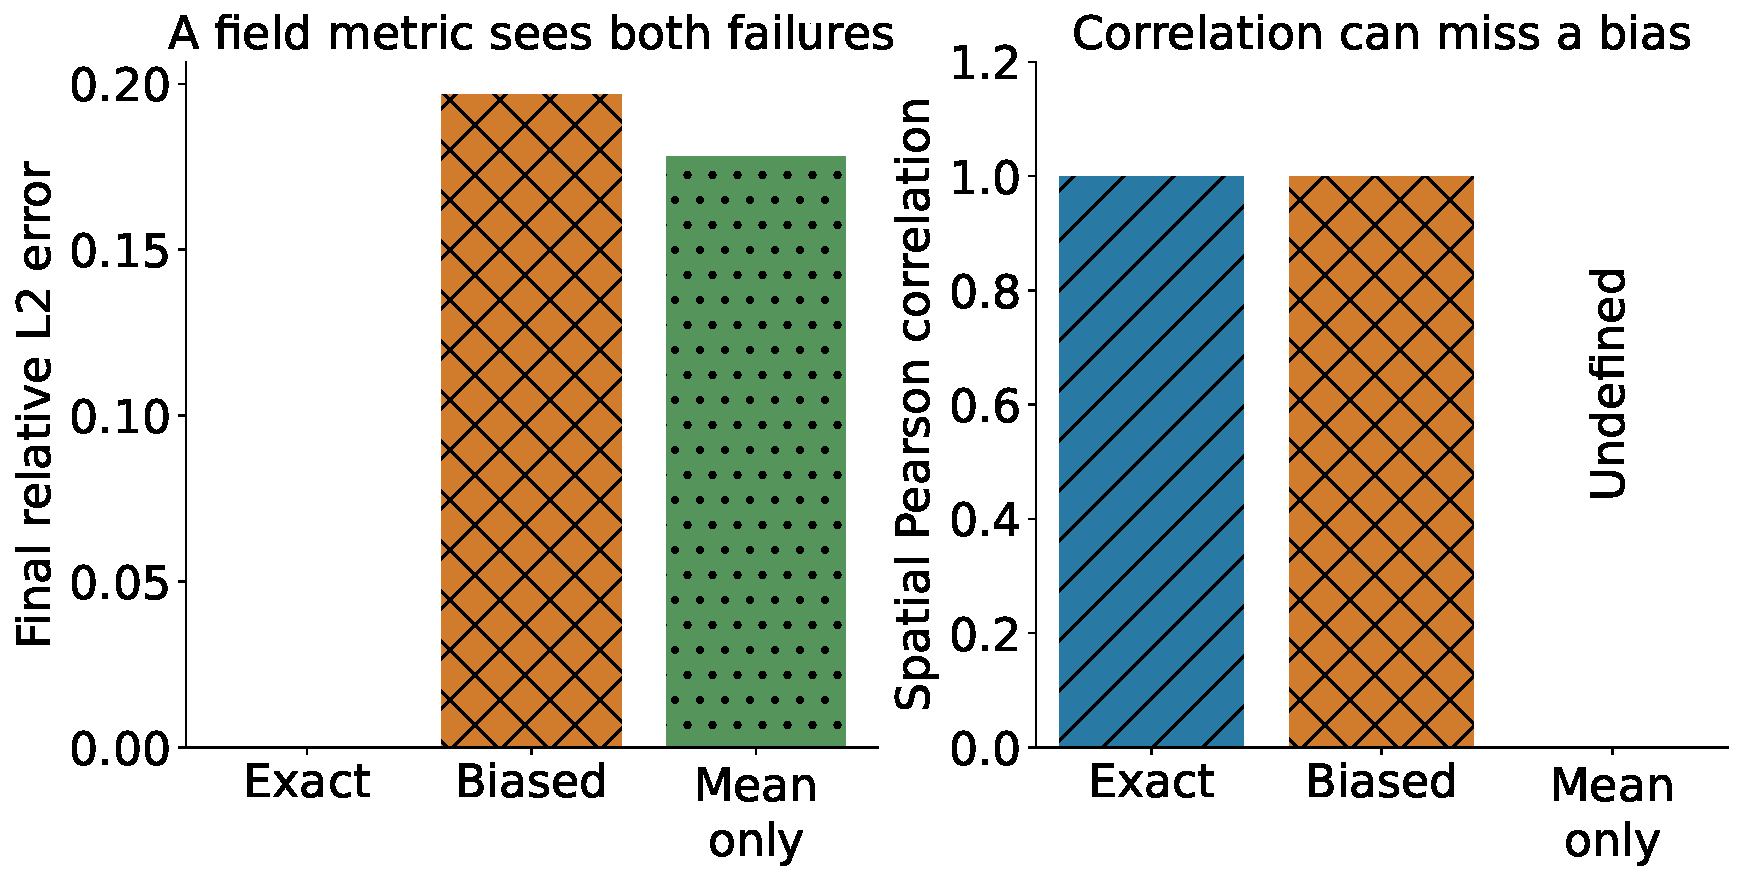
\includegraphics[width=.96\linewidth,height=.57\textheight,keepaspectratio]{evidence-audit.pdf}\par\smallskip
{\small Original final-time field errors and spatial correlations. An additive bias leaves correlation near one; a constant candidate has undefined correlation and is labeled accordingly.}
\end{minipage}\end{center}
\section{Affine invariance of Pearson correlation}
\hypertarget{note-affine-invariance-of-pearson-correlation}{}\label{note:affine-invariance-of-pearson-correlation}
{\small \href{slides.html\#frame=pearson-correlation\&step=1}{Slides for this section}}\par
Pearson correlation subtracts each vector's mean, takes the dot product of the centered vectors, and divides by their centered norms. Adding a constant to a nonconstant vector disappears during centering. Multiplying it by a positive constant scales numerator and denominator equally. Therefore a positively rescaled and shifted prediction can have correlation one while its absolute values are wrong. Negative rescaling reverses the correlation sign, but neither sign alone quantifies amplitude error.

For a concrete calculation, take reference values 1,3,5 and a prediction shifted upward by 2. Both centered vectors are\ensuremath{-}2,0,2, so their correlation is one. The error vector is 2,2,2, giving RMS error 2 and mean error 2. These statements are compatible: correlation answers a centered-pattern question, while RMS and mean error detect the offset. Calling the first result accurate without specifying the metric would hide the failure.

The GFuNK paper reports multiple metrics and explicitly notes the offset and positive-rescaling invariance of correlation. Our lesson derives that property and tests it on new synthetic values; it does not reinterpret the paper's reported performance as a clinical validation result. In a scientific talk, show the metric definitions and choose them according to the intended observable, not according to which produces the most favorable number.

\[
\rho(p,y)=\frac{(p-\bar p\mathbf1)^T(y-\bar y\mathbf1)}{\|p-\bar p\mathbf1\|\,\|y-\bar y\mathbf1\|}
\]
Both centered norms must be nonzero. Additive offsets and positive rescaling leave correlation unchanged.

Let $p=ay+b\boldsymbol1$ and assume $y$ is nonconstant. Centering gives $p-\bar p\boldsymbol1=a(y-\bar y\boldsymbol1)$. Therefore
\[
 \rho(p,y)=\frac{a\|y-\bar y\boldsymbol1\|^2}{|a|\|y-\bar y\boldsymbol1\|^2}
 =\operatorname{sign}(a),\qquad a\ne0.
\]
For $a>0$, correlation is one regardless of offset or amplitude error. If $a=0$, the prediction is constant and its centered norm vanishes, so correlation is undefined.

\paragraph{Calculation.} Compare y=[1,3,5] with p=[3,5,7].

Both centered vectors are[\ensuremath{-}2,0,2], so their normalized dot product is 1.

The pointwise error is[2,2,2], giving RMS error 2.

The prediction mean is 5 while the reference mean is 3, so mean error is 2.

Perfect correlation does not establish correct amplitude or offset.
\section{Conservation and prescribed initial data}
\hypertarget{note-conservation-and-prescribed-initial-data}{}\label{note:conservation-and-prescribed-initial-data}
{\small \href{slides.html\#frame=conservation-relative-to-the-initial-prediction-panel-1\&step=1}{Slides for this section}}\par
The exact sealed heat solution preserves its initial mean. The biased candidate also preserves its own mean, but starts from the wrong mean. A test that compares each candidate only with its own initial average would accept both. The correct audit includes consistency with the prescribed initial field, not merely constancy of an internal quantity. This is the same reason a circulation model needs the intended total blood volume rather than an arbitrary conserved total.

The mean-only candidate creates a different failure. It matches the prescribed mean at every time and therefore passes that aggregate balance. Yet it discards the nonconstant input modes, including at the initial time. Its initial-condition mismatch and spatial field error expose the defect. A conservation test is still valuable; it simply constrains one aspect of the computation rather than certifying the entire trajectory.

The figure shows final fields beside their mean histories. Read the two panels together. Identical mean histories can accompany different spatial profiles, while a flat mean history can be consistently offset from the prescribed value. A good presentation should state exactly which budget is verified, which initial or boundary data were used and which independent observable is needed to assess the rest of the claim.

Two separate residuals distinguish drift from initial-condition mismatch:
\[
 r_{drift}(t)=\overline p(t)-\overline p(0),\qquad
 r_{prescribed}(t)=\overline p(t)-\overline y(0).
\]
For $p=y+b$, the first is zero under sealed heat flow while the second equals $b$. Conservation of an incorrect initial mean is an exact but irrelevant invariant for the prescribed problem.
\begin{center}\begin{minipage}{.98\linewidth}\centering
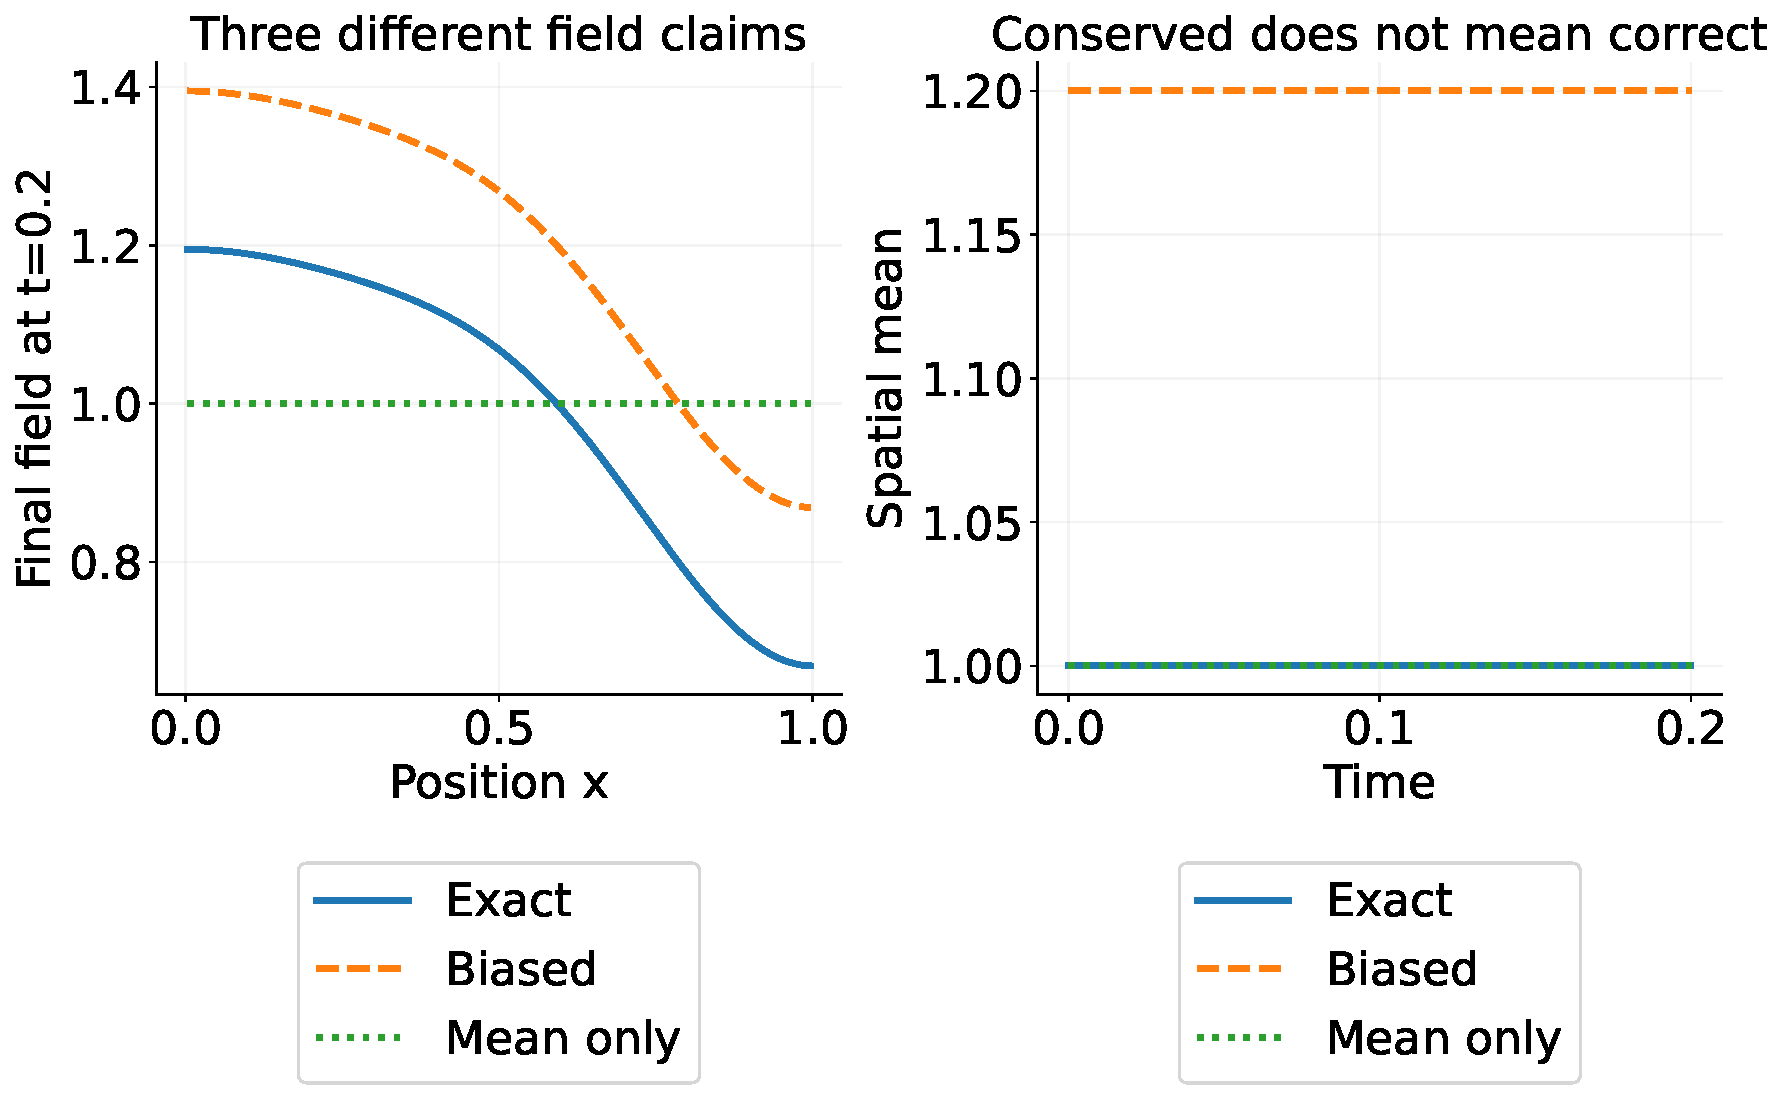
\includegraphics[width=.96\linewidth,height=.57\textheight,keepaspectratio]{field-and-moment.pdf}\par\smallskip
{\small Original synthetic heat reference, additive-bias candidate and mean-only candidate. Each conserves its own mean, but that fact alone misses initial-state bias or lost spatial structure.}
\end{minipage}\end{center}
\section{Orthogonal error components}
\hypertarget{note-orthogonal-error-components}{}\label{note:orthogonal-error-components}
{\small \href{slides.html\#frame=orthogonal-decomposition-of-field-error\&step=1}{Slides for this section}}\par


Decompose the error orthogonally as $e=\bar e\boldsymbol1+e_c$, where $\boldsymbol1^{\mathsf T}e_c=0$. The cross term vanishes, giving
\[
 \frac1N\|e\|^2=\bar e^2+\frac1N\|e_c\|^2.
\]
A mean measurement constrains only the first term. A constant mean-only prediction can set that term to zero while losing every nonconstant mode. Correlation normalizes centered patterns and therefore does not recover their amplitude. These statements explain why the metrics complement one another rather than compete for a single preferred score.
\section{Synthesis across models and representations}
\hypertarget{note-synthesis-across-models-and-representations}{}\label{note:synthesis-across-models-and-representations}
{\small \href{slides.html\#frame=a-precise-synthesis\&step=1}{Slides for this section}}\par


The known heat examples separate numerical defects from limitations of an observable. An offset field fails the prescribed mean while retaining perfect correlation. A mean-only field preserves that aggregate but loses spatial structure. Similar distinctions recur in the circulation, shape and wave problems: a conserved total does not identify its distribution, a fitted pose does not establish correspondence, and a threshold time does not determine the full waveform. A supported conclusion is the mathematical property demonstrated under the stated assumptions, together with the quantities that remain undetermined.
\bigskip
\section*{Exercises}
\par\noindent\begin{minipage}{\linewidth}
\subsection*{E1. Perfect correlation with a bias}
Let y=\allowbreak{}[1,2,3] and p=\allowbreak{}[2,3,4].

\textbf{a} Calculate Pearson correlation, RMS error and mean error.

\end{minipage}\par\medskip
\textbf{b} Calculate relative L$^2$ error and write an accurate result statement.

\par\noindent\begin{minipage}{\linewidth}
\subsection*{E2. An exact mean with lost structure}
Reference y=\allowbreak{}[0,2,0,2] and candidate p=\allowbreak{}[1,1,1,1].

\textbf{a} Compute the mean error and relative L$^2$ field error.

\end{minipage}\par\medskip
\textbf{b} What is the candidate's Pearson correlation with the reference? How should it be reported?

\par\noindent\begin{minipage}{\linewidth}
\subsection*{E3. Review a conservation claim}
A presenter says: Every run conserves its own mean, therefore the solver is correct.

\textbf{a} Give two counterchecks that directly address the claim.

\end{minipage}\par\medskip
\textbf{b} Rewrite the claim in a defensible form.

\par\noindent\begin{minipage}{\linewidth}
\subsection*{E4. Plan a short scientific presentation}
Use any one verified result from the course; do not invent experimental evidence.

\textbf{a} Give a five-part outline that a reviewer can assess.

\end{minipage}\par\medskip
\textbf{b} Write one actionable peer-review question and explain what its answer could change.

\section*{References}
\noindent\begin{minipage}{\linewidth}
Zan Ahmad, Advanced Topics in Computational Cardiology syllabus, Fall 2024. PDF pages 1--2.

\end{minipage}\par\medskip
\noindent\begin{minipage}{\linewidth}
Loeffler, Ahmad, Chen and collaborators, Graph Fourier Neural Kernels: Learning Full PDE Trajectories Across Geometries and Anisotropic Parameter Fields. Main text section 2.3, printed/PDF pages 10--11: field and correlation metrics; section 3, pages 12--13: limitations.

\end{minipage}\par\medskip
\end{document}
